%!TEX root = ../PRESENTATION_DGA.tex
\documentclass[11pt,class=book]{standalone}
%\usepackage[utf8]{inputenc}
\usepackage[french]{babel}
\usepackage[french]{translator}
\usepackage[T1]{fontenc}
\usepackage{fontspec}
\usepackage[table,svgnames]{xcolor}

\usepackage{pgf}
\usepackage{tikz}

\usepackage{array}
\usepackage{tabularx}
\usepackage{multirow}
\usepackage{pgf-umlsd}
\usepackage{pgfgantt}

\usetikzlibrary{shapes}
\usetikzlibrary{arrows.meta}
\usetikzlibrary{calc}

\definecolor{bg_color}{RGB}{250,250,229}

\colorlet{color1}{cyan!50}
\colorlet{color2}{red!30!green!40}
\colorlet{color3}{orange!50}
\colorlet{color4}{violet!60!blue!55}

\newganttlinktype{bartobardown}{
	\ganttsetstartanchor{south east}
	\ganttsetendanchor{north west}
	\draw [/pgfgantt/link] (\xLeft, \yUpper) -- (\xRight, \yLower);
}
\newganttlinktype{bartobarup}{
	\ganttsetstartanchor{north east}
	\ganttsetendanchor{south west}
	\draw [/pgfgantt/link] (\xLeft, \yUpper) -- (\xRight, \yLower);
}
\newganttlinktype{milestonetobardown}{
	\ganttsetstartanchor{south}
	\ganttsetendanchor{north west}
	\draw [/pgfgantt/link] (\xLeft, \yUpper) -- (\xRight, \yLower);
}
\newganttlinktype{bartomilestonedown}{
	\ganttsetstartanchor{south east}
	\ganttsetendanchor{north}
	\draw [/pgfgantt/link] (\xLeft, \yUpper) -- (\xRight, \yLower);
}


\begin{document}
	\begin{tikzpicture}[x=1pt,y=1pt]
		\tikzset{zone/.style={
			thick,
			inner sep=0,
			outer sep=0,
			fill opacity=0.25
		}}
		\tikzset{txt/.style={
			black,
			fill opacity=1,
			font=\bf
		}}

		\node[
			anchor=south west,
			inner sep=0
		] (image) at (0,0)
		{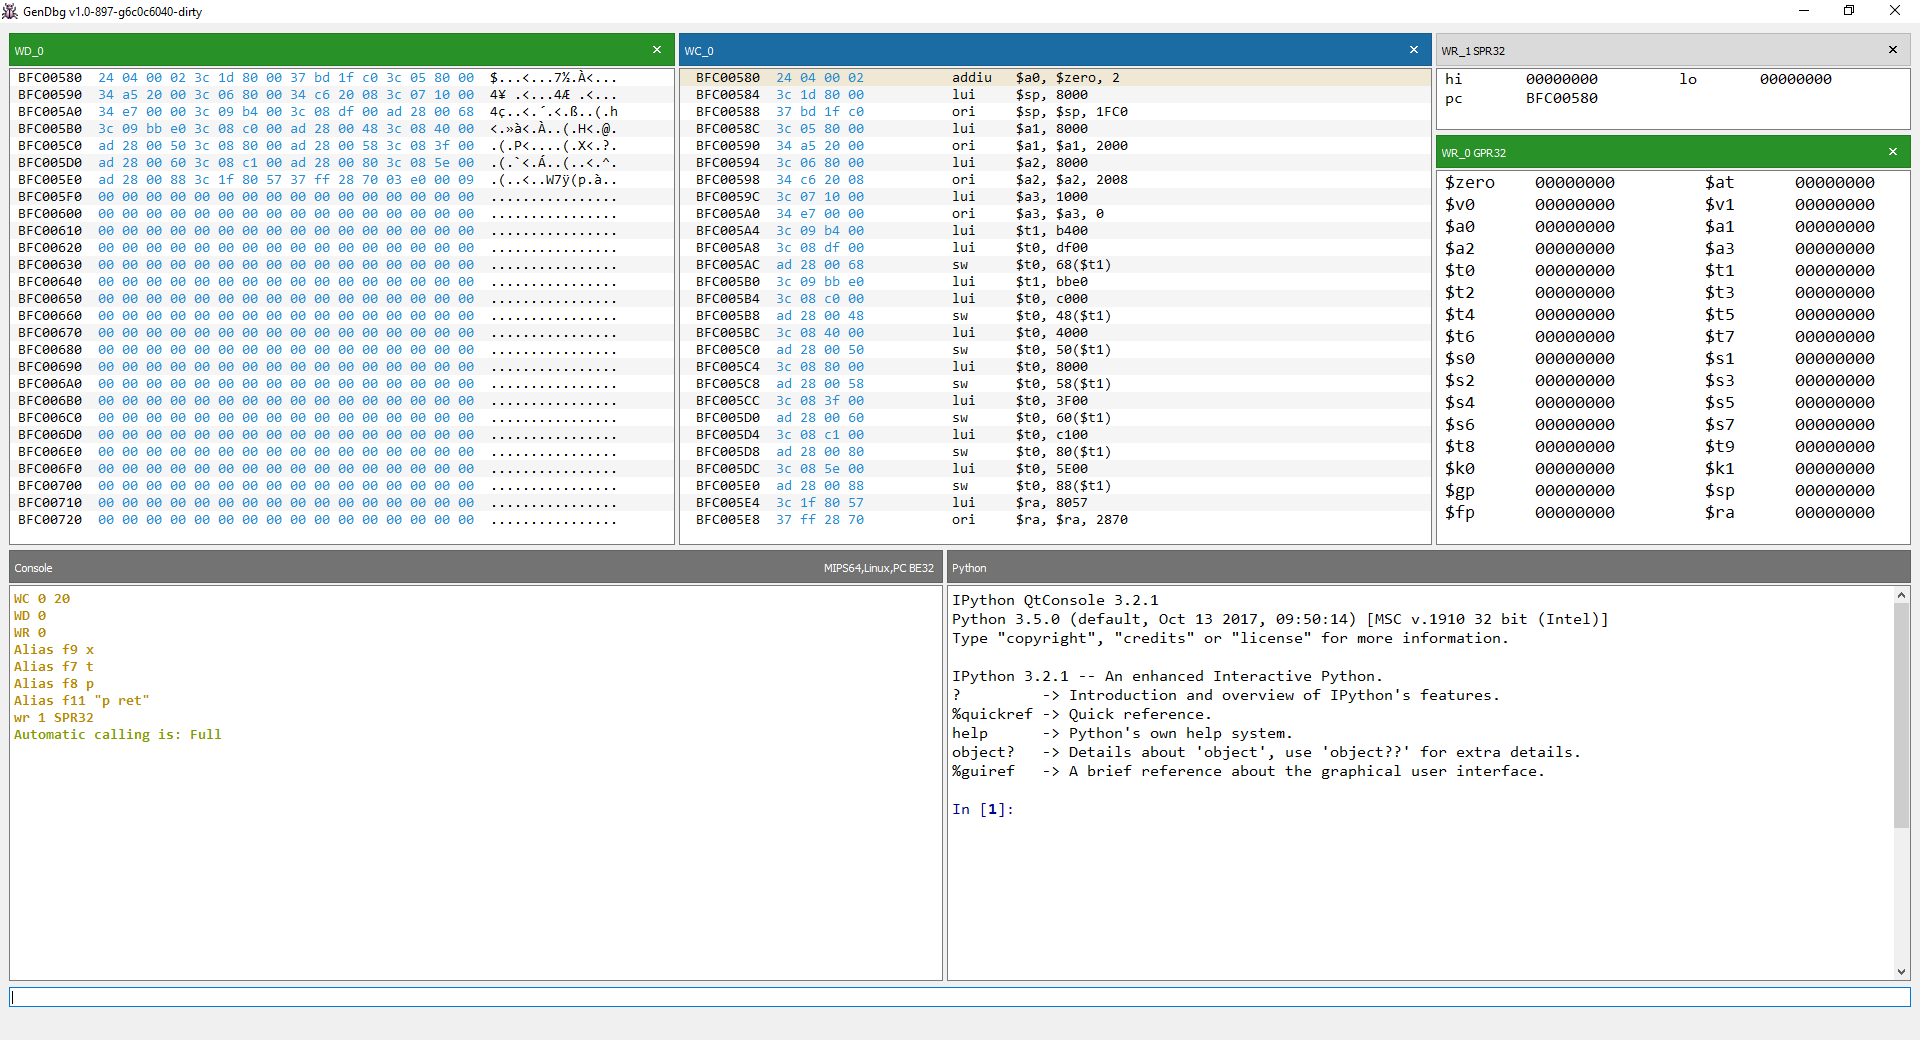
\includegraphics[width=0.9\textwidth]{GenDbg_GUI_Qt}};

		\begin{scope}[x={(image.south east)},y={(image.north west)}]
			%\draw[help lines,xstep=.1,ystep=.1] (0,0) grid (1,1);
			%\foreach \x in {0,1,...,9} { \node [anchor=north] at (\x/10,0) {\tiny 0.\x}; }
			%\foreach \y in {0,1,...,9} { \node [anchor=east] at (0,\y/10) {\tiny 0.\y}; }
			\uncover<2>{
				\draw[
					zone,
					green,
					fill=green
				] (0.0054,0.97) rectangle
					node[txt] {Vue Hexa}
				(0.3515,0.4765);
			}
			\uncover<2,3>{
				\draw[
					zone,
					blue,
					fill=blue
				] (0.3545,0.97) rectangle
					node[txt] {Vue Code}
				(0.745,0.4765);
			}
			\uncover<2>{
				\draw[
					zone,
					red,
					fill=red
				] (0.748,0.97) rectangle
					node[txt] {Registres}
				(0.995,0.4765);
			}
			\uncover<2>{
				\draw[
					zone,
					red,
					fill=red
				] (0.0054,0.471) rectangle
					node[txt] {Console classique}
				(0.491,0.0565);
			}
			\uncover<2>{
				\draw[
					zone,
					green,
					fill=green
				] (0.494,0.471) rectangle
					node[txt] {Console Python}
				(0.995,0.0565);
			}
		\end{scope}
	\end{tikzpicture}
\end{document}
